\documentclass[xcolor=x11names, svgnames, rgb]{beamer}

\setbeamertemplate{navigation symbols}{}
\setbeamercolor{block title}{bg=blue!40}
\setbeamercolor{block body}{bg=blue!20}

%% Beamer Layout %%%%%%%%%%%%%%%%%%%%%%%%%%%%%%%%%%
\useoutertheme[subsection=false,shadow]{miniframes}
\useinnertheme{default}
\usefonttheme{serif}
\usepackage{palatino}
\setbeamerfont{title like}{shape=\scshape}
\setbeamerfont{frametitle}{shape=\scshape}
\setbeamercolor*{lower separation line head}{bg=DeepSkyBlue4}
\setbeamercolor*{normal text}{fg=black,bg=white}
\setbeamercolor*{alerted text}{fg=red}
\setbeamercolor*{example text}{fg=black}
\setbeamercolor*{structure}{fg=black}
\setbeamercolor*{palette tertiary}{fg=black,bg=black!10}
\setbeamercolor*{palette quaternary}{fg=black,bg=black!10}
%% END Beamer Layout %%%%%%%%%%%%%%%%%%%%%%%%%%%%%%%%%%%%%%%%%%%%
\usepackage{graphicx}
\usepackage{algpseudocode}
\usepackage{soul}

\usepackage{mathtools}
\newcommand{\defeq}{\vcentcolon=}
\DeclarePairedDelimiter{\paren}{(}{)}

\newcommand{\dec}{\operatorname{dec}}
\newcommand{\poly}{\operatorname{poly}}
\newcommand{\polylog}{\operatorname{polylog}}
\newcommand{\github}{\url{github.com/awestover/Parallel-Partition}}
\newcommand{\defn}[1]       {{\textit{\textbf{\boldmath #1}}}}
\newcommand{\paragraph}[1]{\vspace{0.09in}\noindent{\bf \boldmath #1.}} 
\usepackage{amsmath}
\def\E{\operatorname{\mathbb{E}}}
\usepackage{amssymb}
\usepackage{amsthm}

\newtheorem{proposition}{Proposition}
\newtheorem{defin}{Definition}

\usepackage{hyperref}

\usepackage{tikz,pgfplots}
\usepackage{etoolbox}
%% This makes the colors annoyingly bright, but at least they're easy to distinguish.
\pgfplotsset{
  every  tick/.style={red,}, minor x tick num=1,
  cycle list={teal,every mark/.append style={fill=teal!80!black},mark=*\\%
orange,every mark/.append style={fill=orange!80!black},mark=square*\\%
cyan!60!black,every mark/.append style={fill=cyan!80!black},mark=otimes*\\%
red!70!white,mark=star\\%
lime!80!black,every mark/.append style={fill=lime},mark=diamond*\\%
red,densely dashed,every mark/.append style={solid,fill=red!80!black},mark=*\\%
yellow!60!black,densely dashed,
every mark/.append style={solid,fill=yellow!80!black},mark=square*\\%
black,every mark/.append style={solid,fill=gray},mark=otimes*\\%
blue,densely dashed,mark=star,every mark/.append style=solid\\%
red,densely dashed,every mark/.append style={solid,fill=red!80!black},mark=diamond*\\%
}
}
\pgfplotsset{compat=1.6}


\usepackage{xcolor}
\newcommand{\citefont}[1]{{\tiny \textcolor{Gray}{#1}}}


\title{Variable Processor Cup Games}
\author{Alek Westover}
\institute{Belmont High School}
\date{June 1, 2020}

\begin{document}
 
\frame{\titlepage}

\begin{frame}[t]{What is the Cup Game?}
  \begin{definition}
  The \defn{$p$-processor cup-game} on $n$ cups is a multi-round game in which
  two players take turns emptying and removing water from the cups. \\
  On each round
  \begin{itemize}
    \item The \defn{filler} distributes $p$ units of water among the cups (with at most $1$ unit to any particular cup). 
    \item Then the \defn{emptier} chooses $p$ cups to remove (at most) one unit of water from.
  \end{itemize}
  \end{definition}
\end{frame}

\begin{frame}[t]{What is the Cup Game?}
  \begin{definition}
  The \defn{backlog} of the system is the amount of water in the fullest cup;
  The emptier aims to minimize backlog whereas the filler aims to maximize
  backlog.
  \end{definition}
  \vspace{0.4cm}

  \textbf{Note:} The emptier's resources must be allocated discretlely whereas
  the filler can continuously distribute resources.
\end{frame}


\begin{frame}[t]{Why is it important?}
  The cup game models \defn{work scheduling}:
  \begin{itemize}
    \item The $n$ cups represent tasks that must be performed. 
    \item At each time step:
      \begin{itemize}
        \item $p$ new units of work come in, distributed
          arbitrarily among the $n$ tasks (with the constraint that no task gets
          more than $1$ unit of work) 
        \item $p$ processors must be allocated to a subset the
          tasks, on which they will achieve $1$ unit of progress.
      \end{itemize}
\end{itemize}

  \vspace{0.5cm}
  The cup game is also an interesting mathematical object.
\end{frame}

\begin{frame}[t]{Single-Processor Lower Bound}
  \textbf{Filling strategy}: distribute water equally amongst cups not yet emptied by the emptier.
  \vspace{0.3cm}

  \begin{overprint}
    \onslide<1>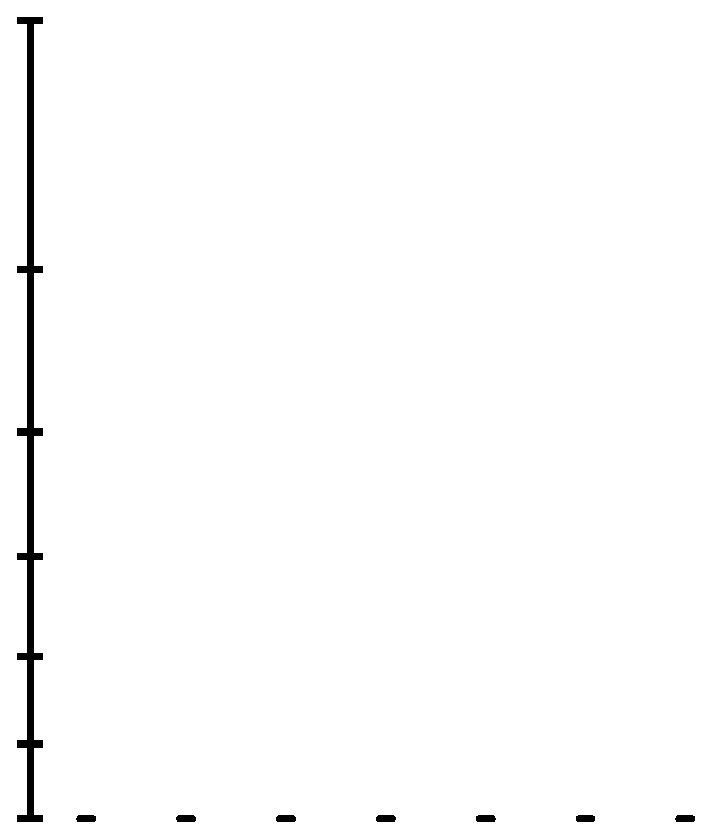
\includegraphics[width=0.5\linewidth]{singleProcessorLowerBound/round_0_1.eps}
    \onslide<2>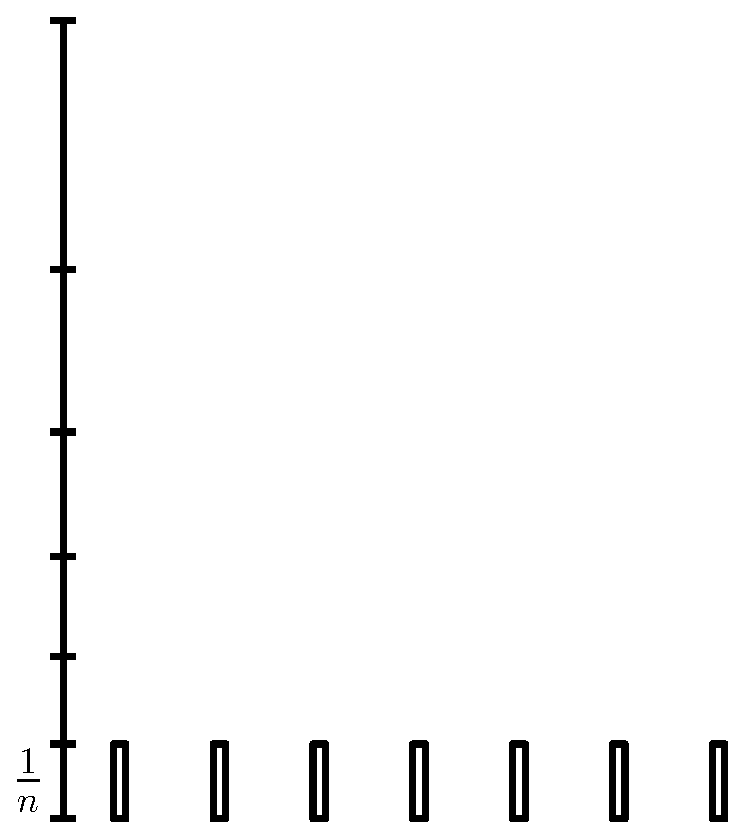
\includegraphics[width=0.5\linewidth]{singleProcessorLowerBound/round_1_0.eps}
    \onslide<3>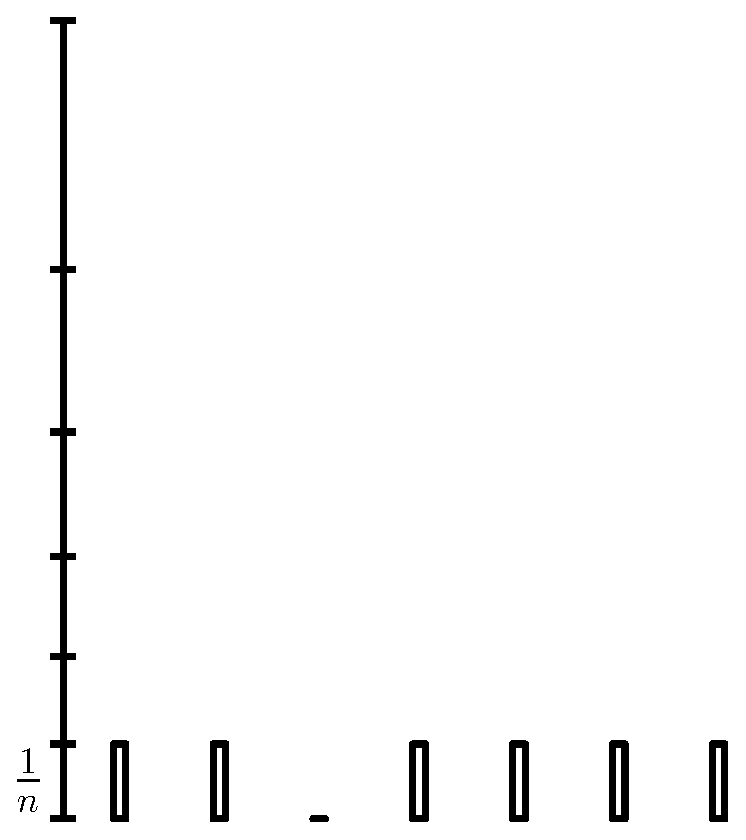
\includegraphics[width=0.5\linewidth]{singleProcessorLowerBound/round_1_1.eps}
    \onslide<4>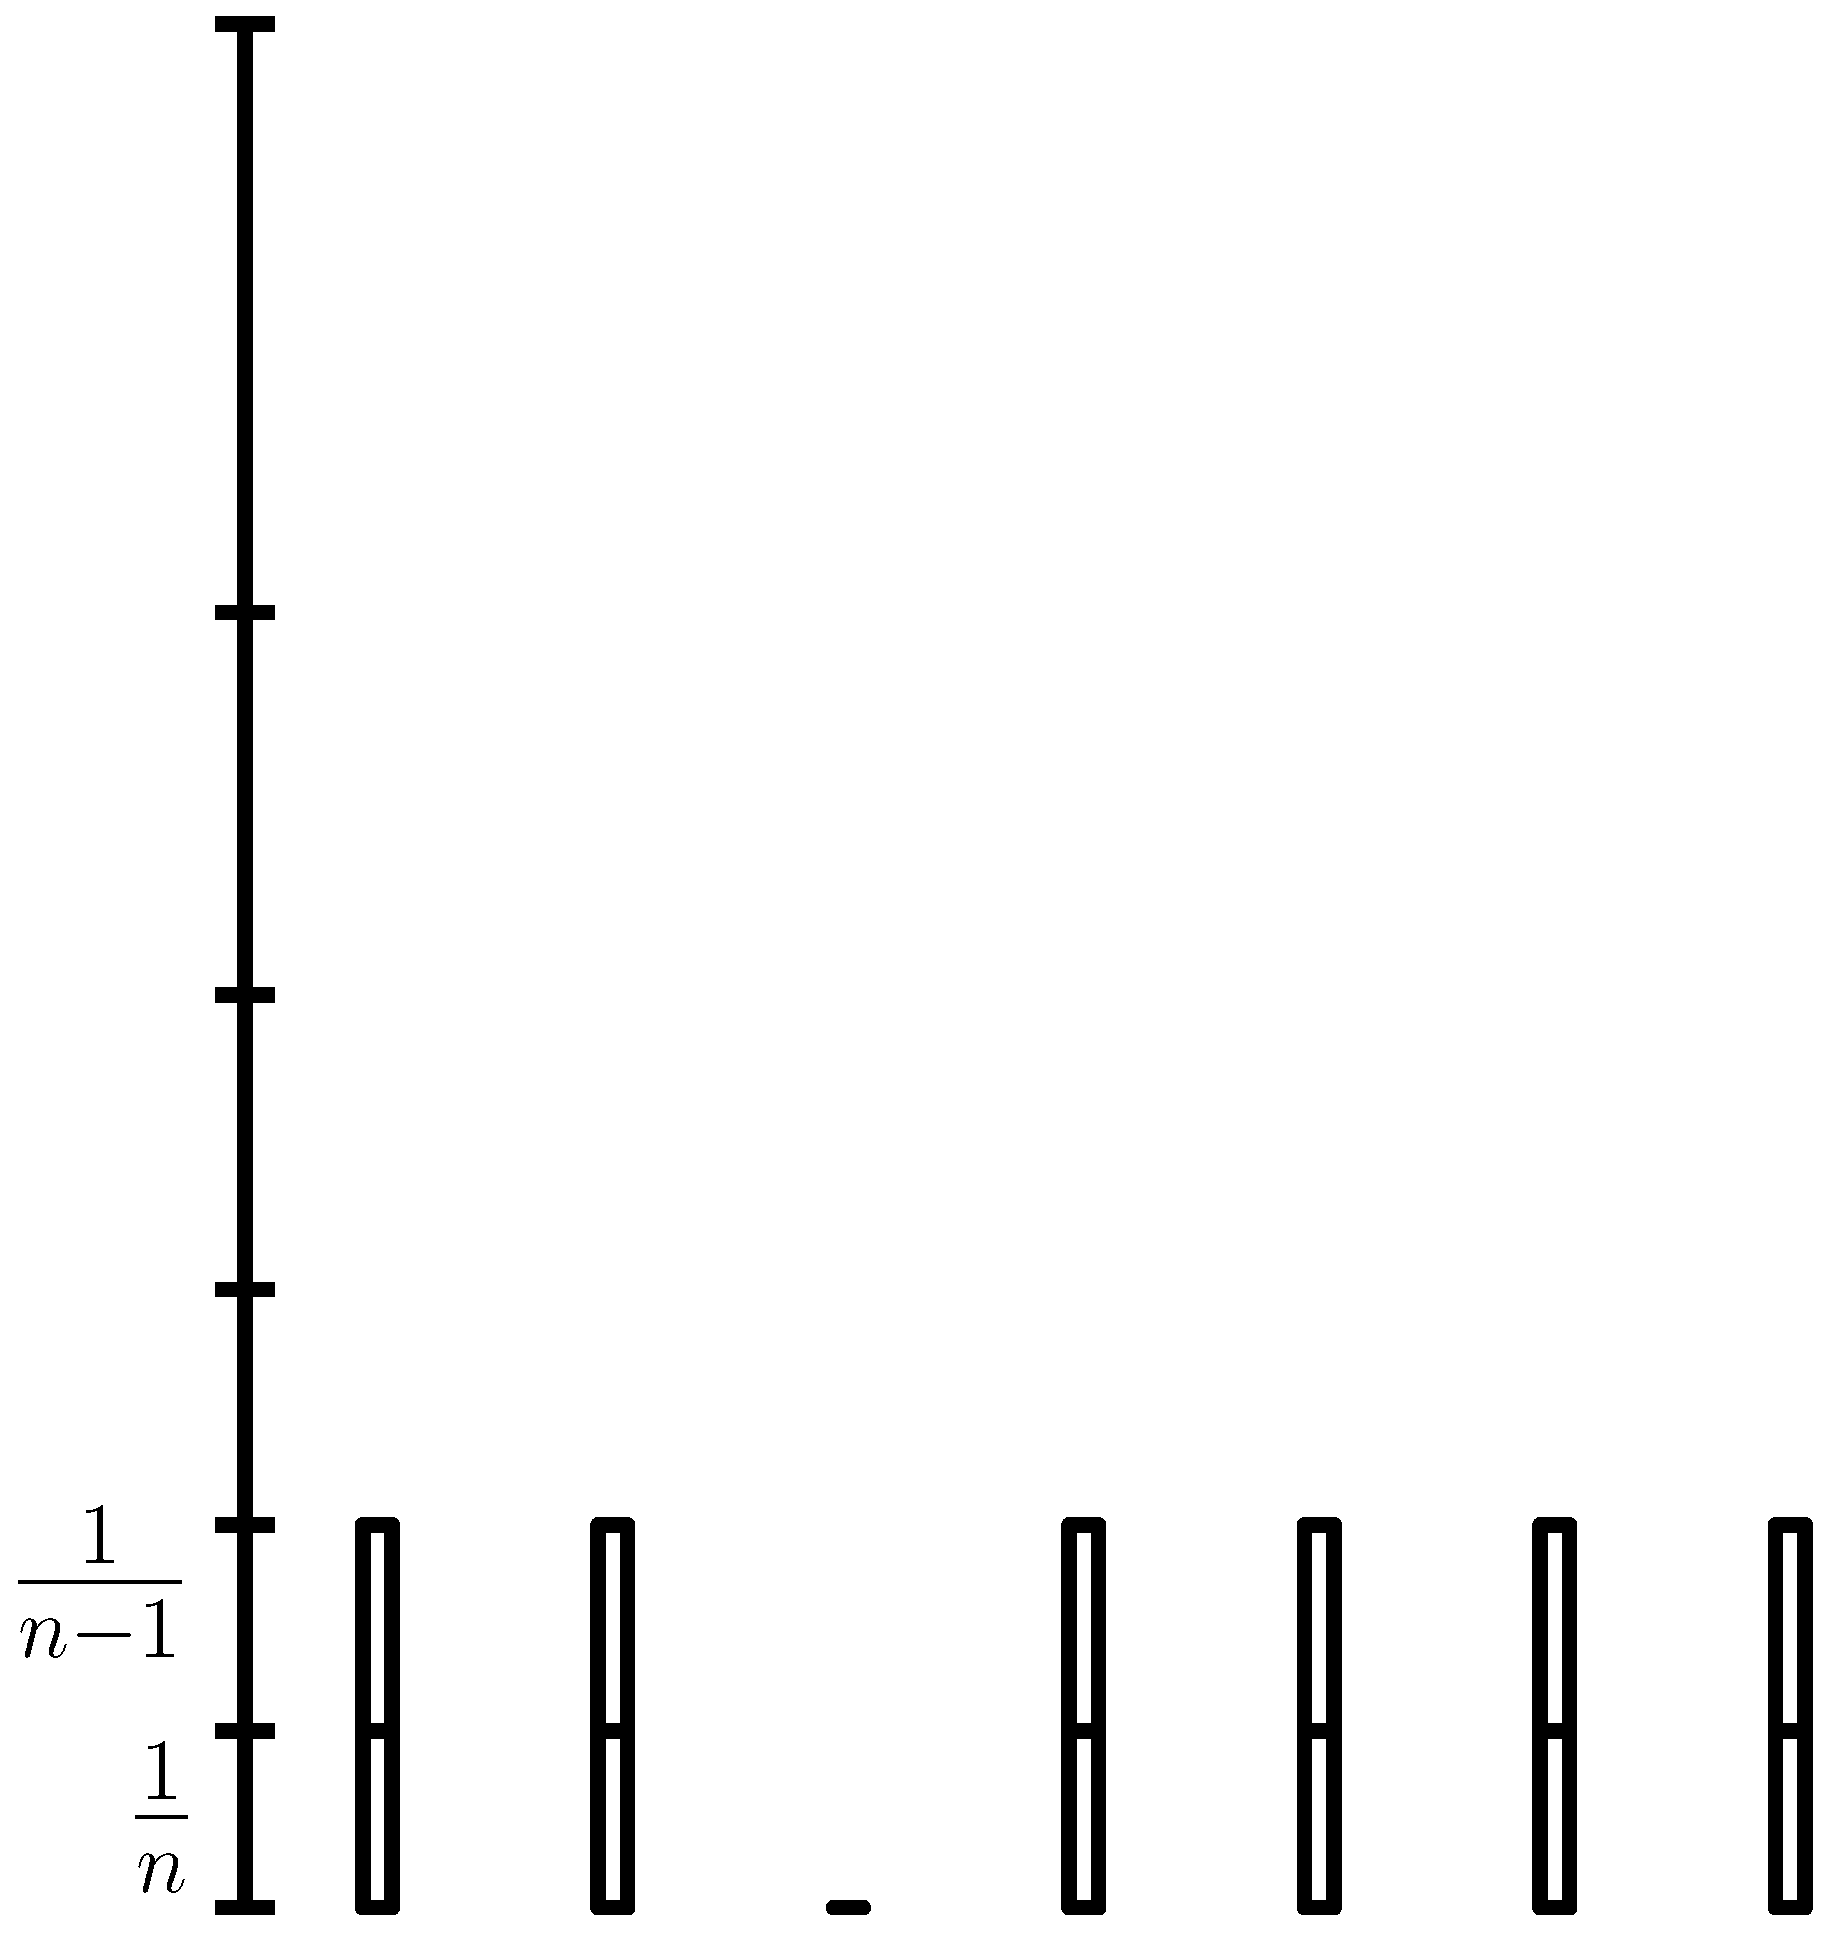
\includegraphics[width=0.5\linewidth]{singleProcessorLowerBound/round_2_0.eps}
    \onslide<5>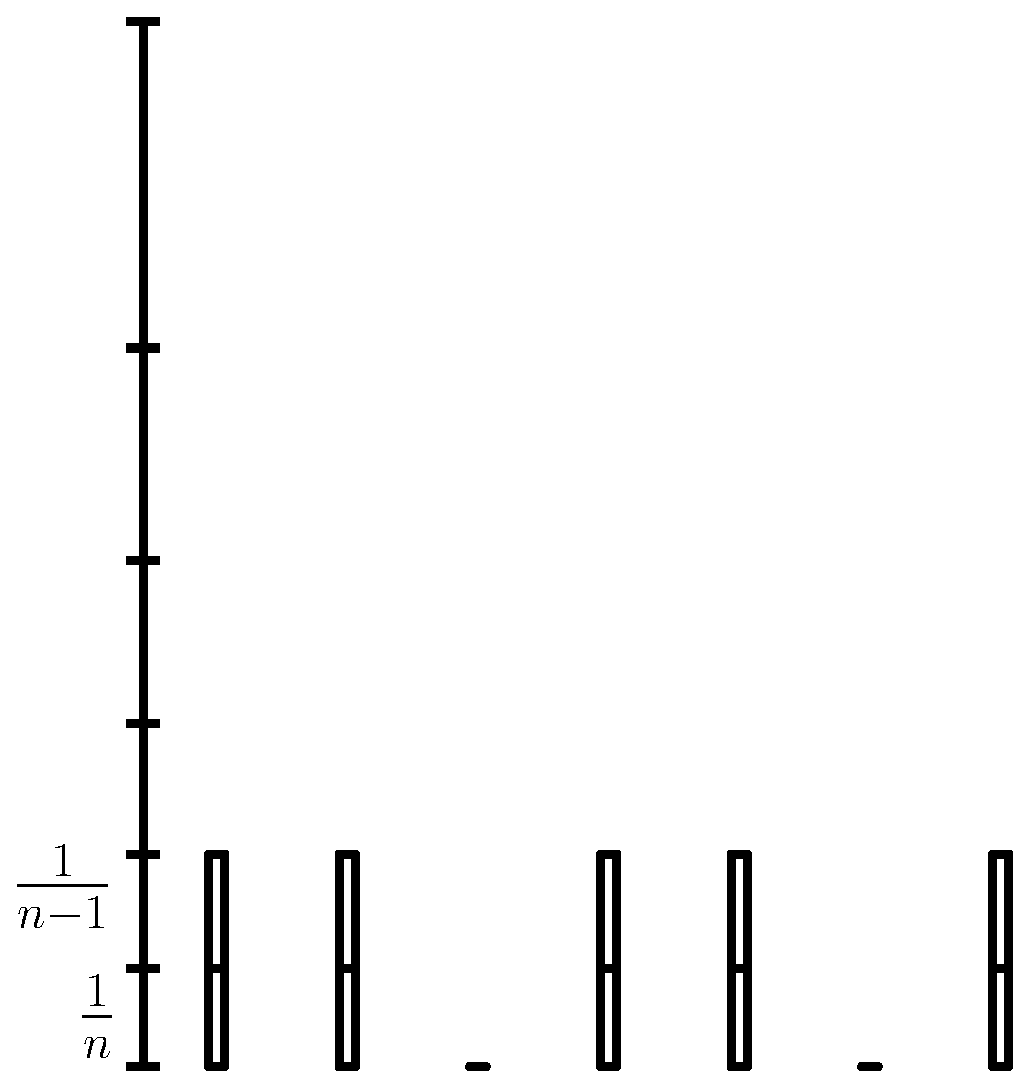
\includegraphics[width=0.5\linewidth]{singleProcessorLowerBound/round_2_1.eps}
    \onslide<6>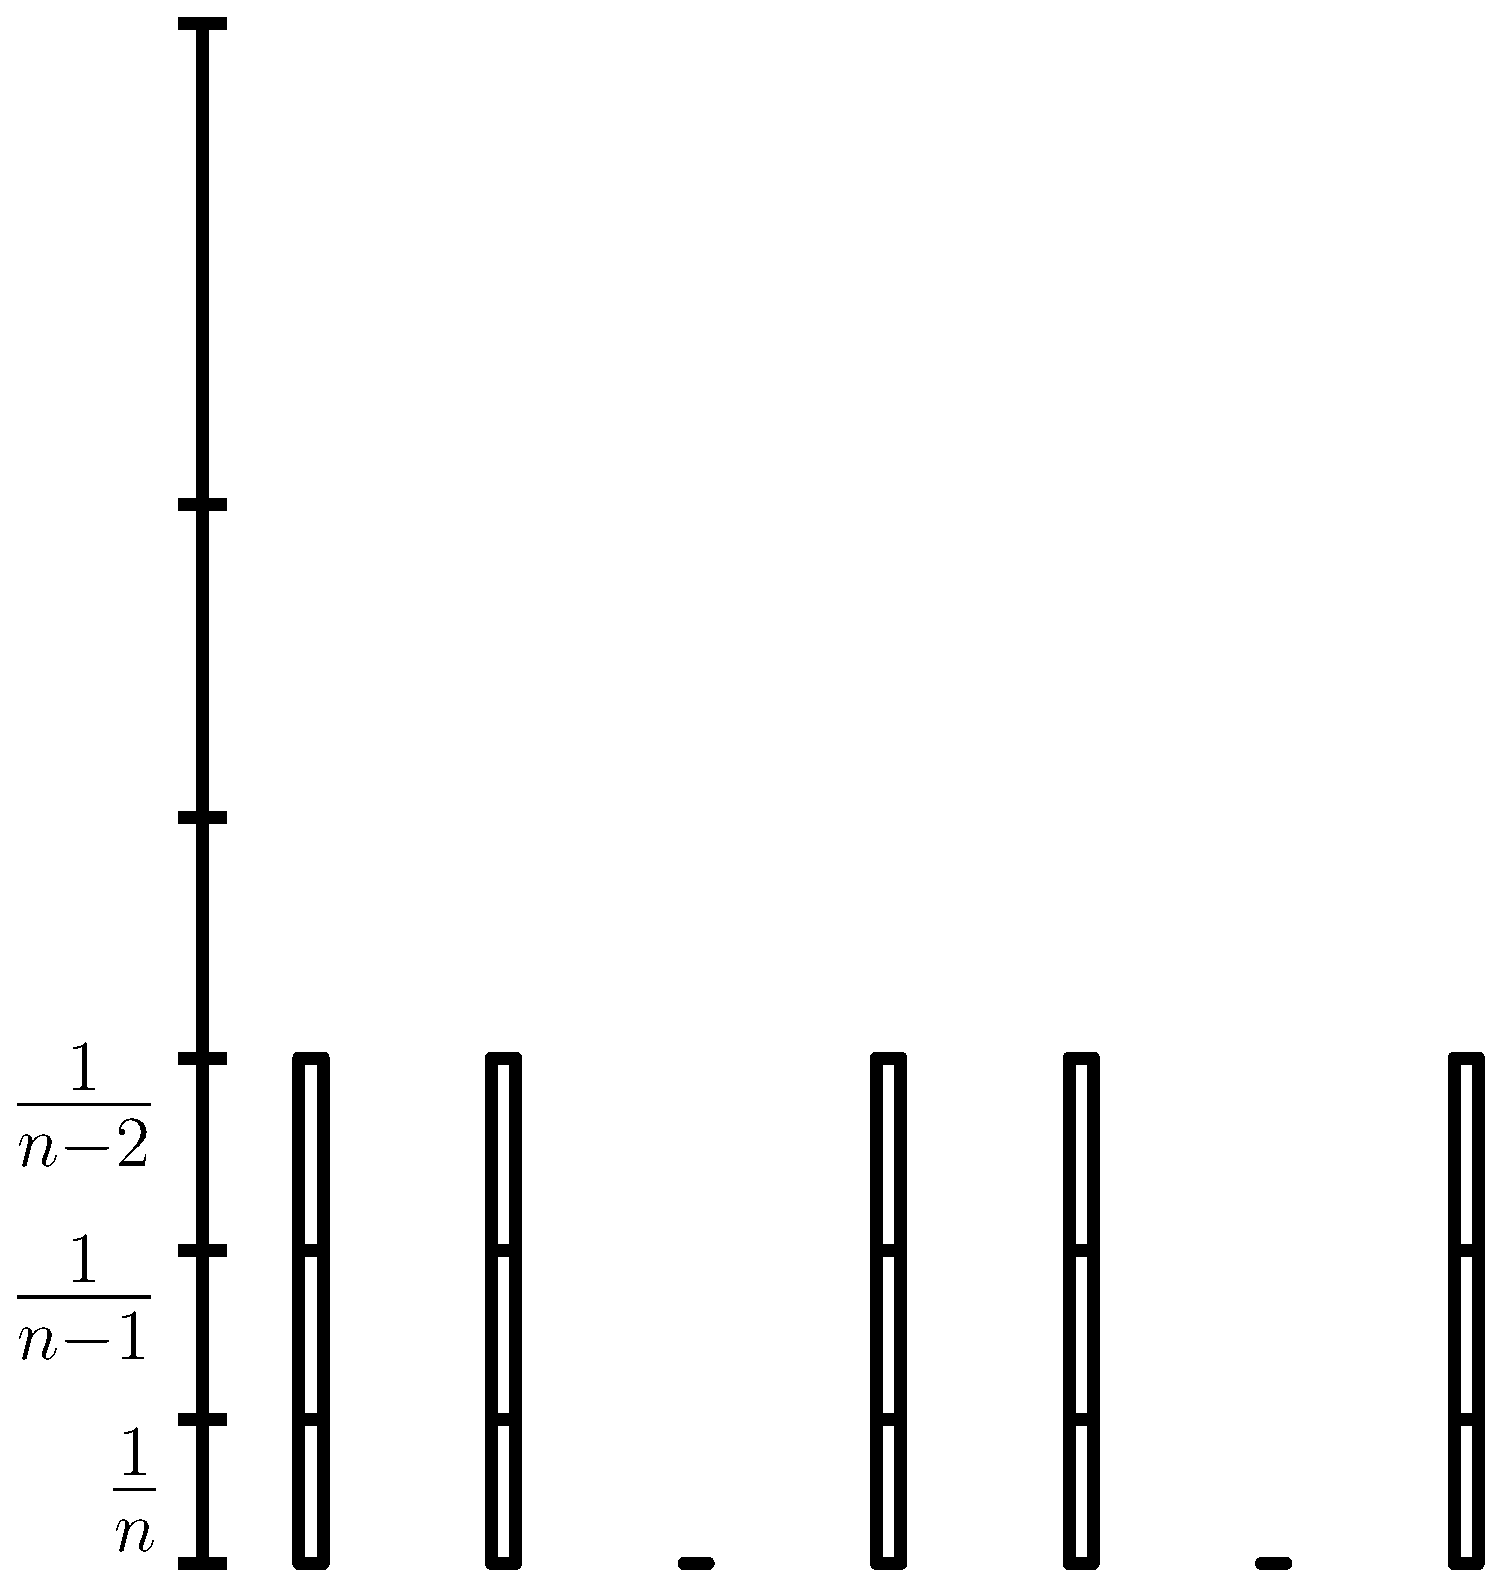
\includegraphics[width=0.5\linewidth]{singleProcessorLowerBound/round_3_0.eps}
    \onslide<7>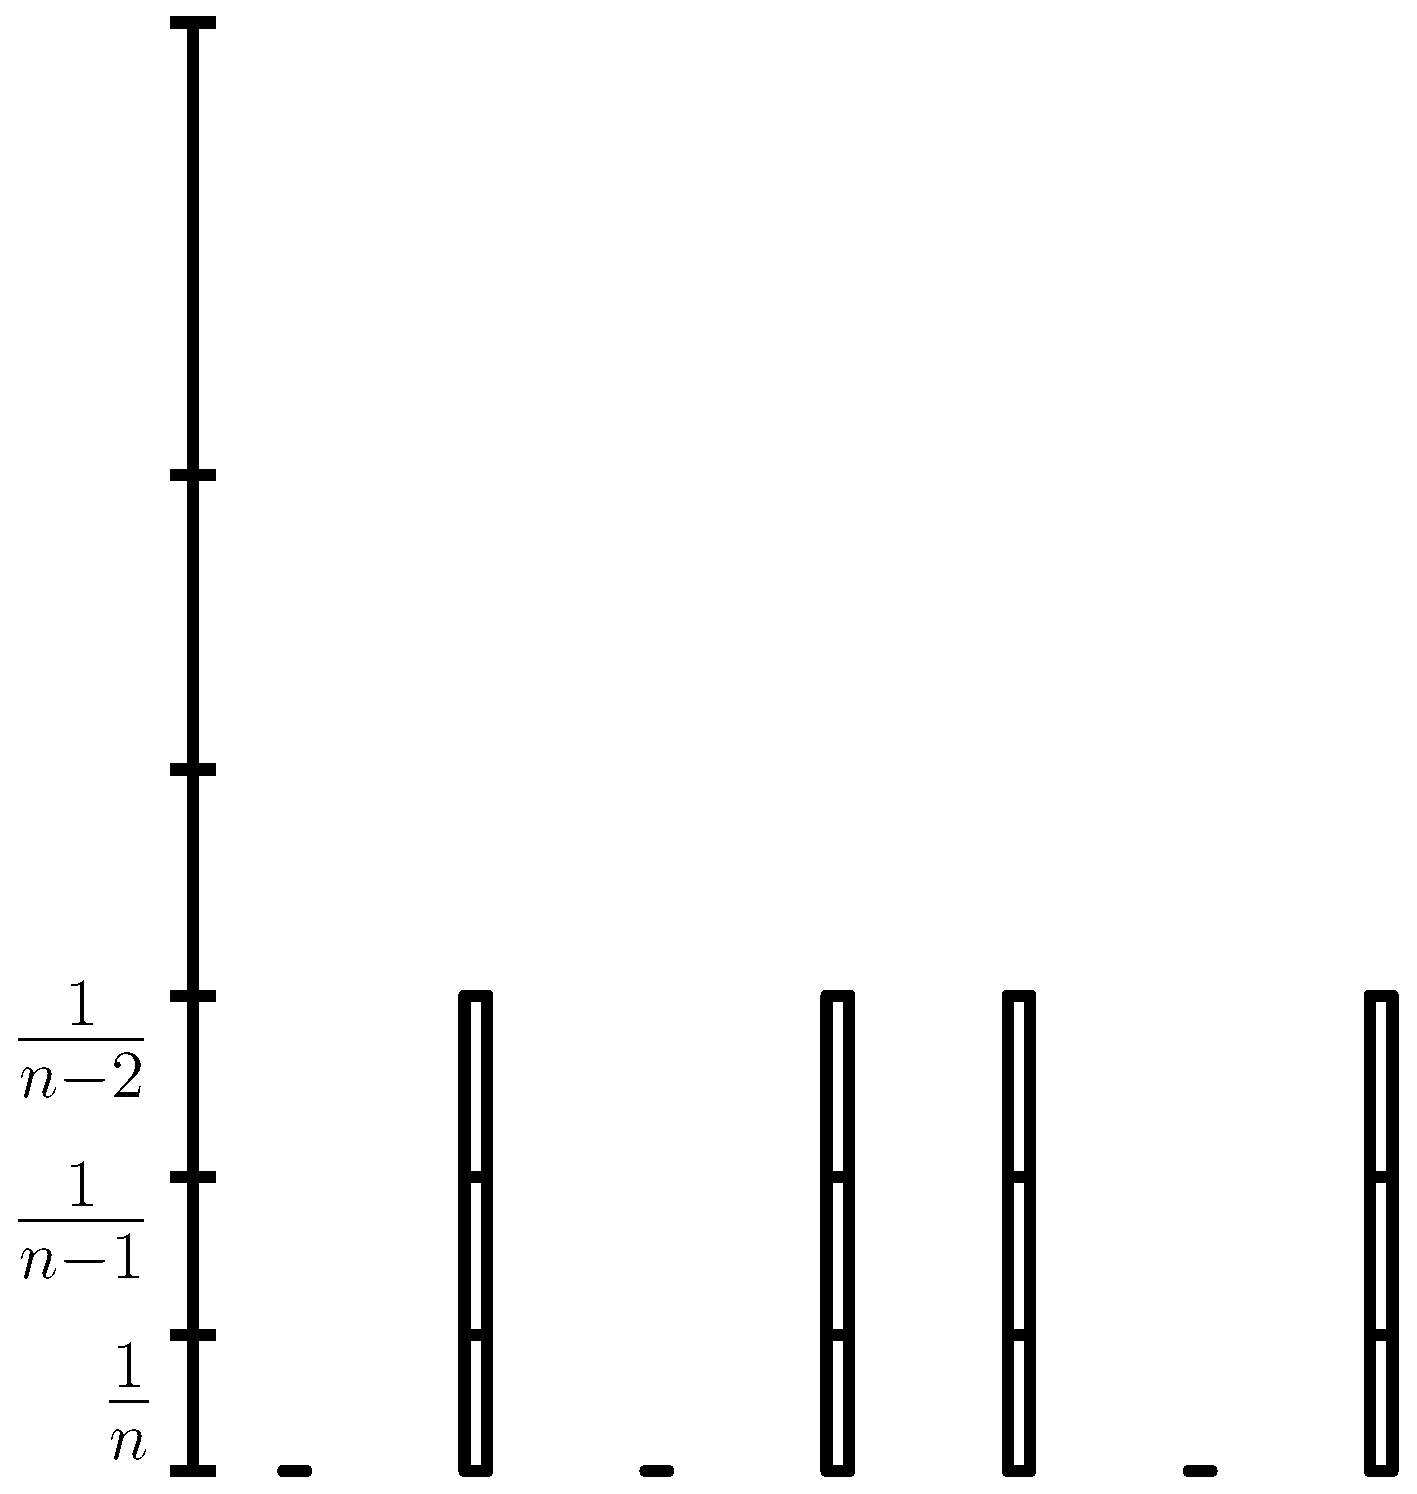
\includegraphics[width=0.5\linewidth]{singleProcessorLowerBound/round_3_1.eps}
    \onslide<8>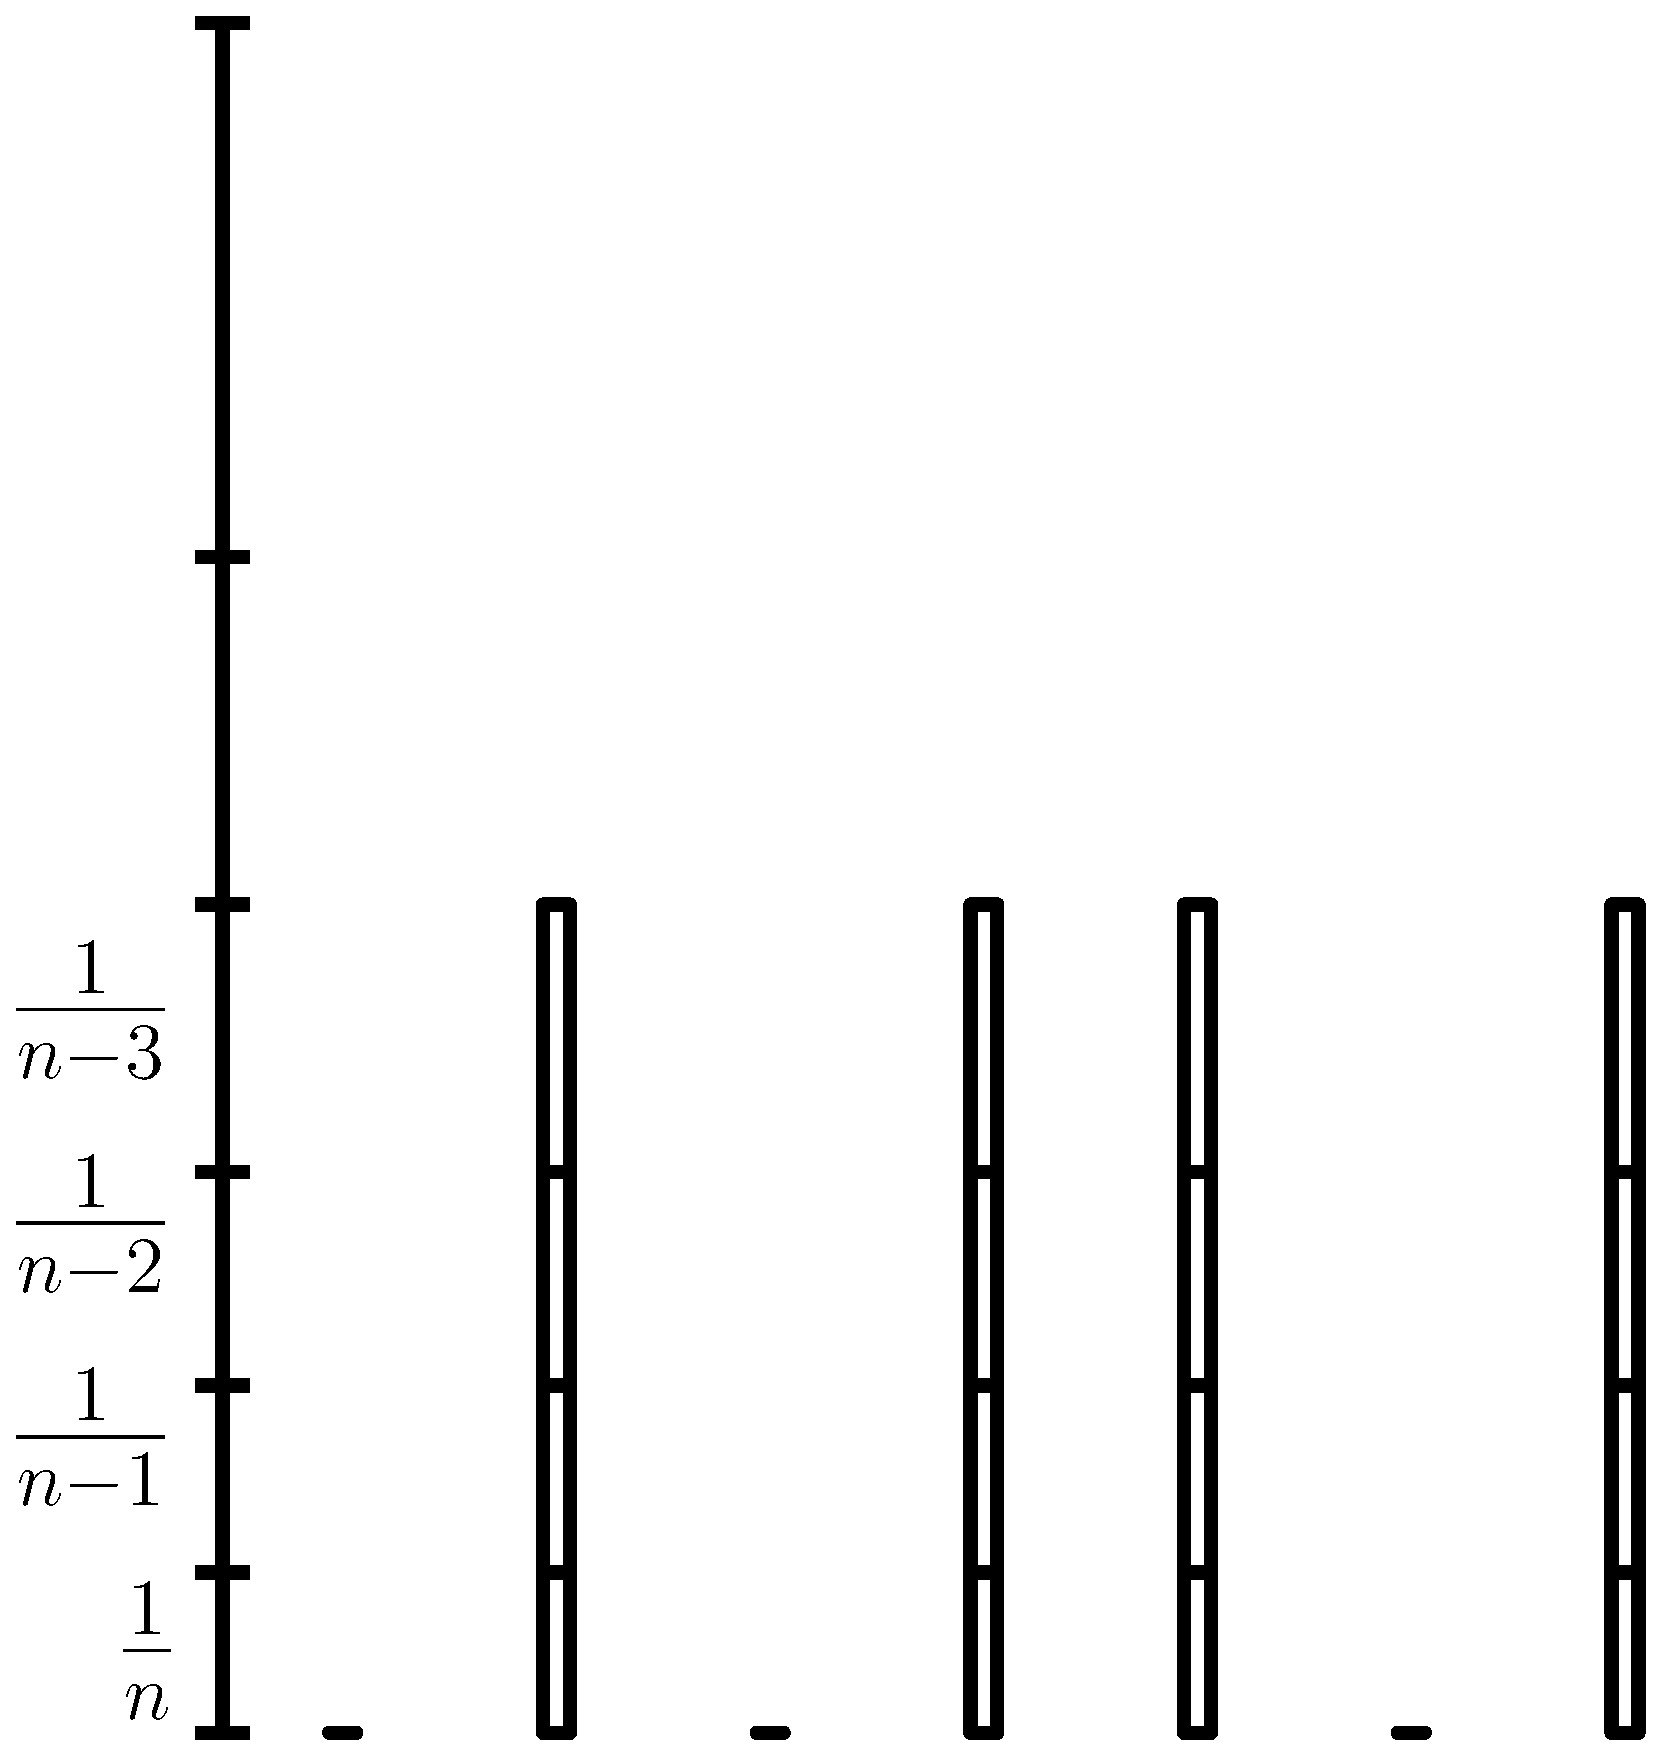
\includegraphics[width=0.5\linewidth]{singleProcessorLowerBound/round_4_0.eps}
    \onslide<9>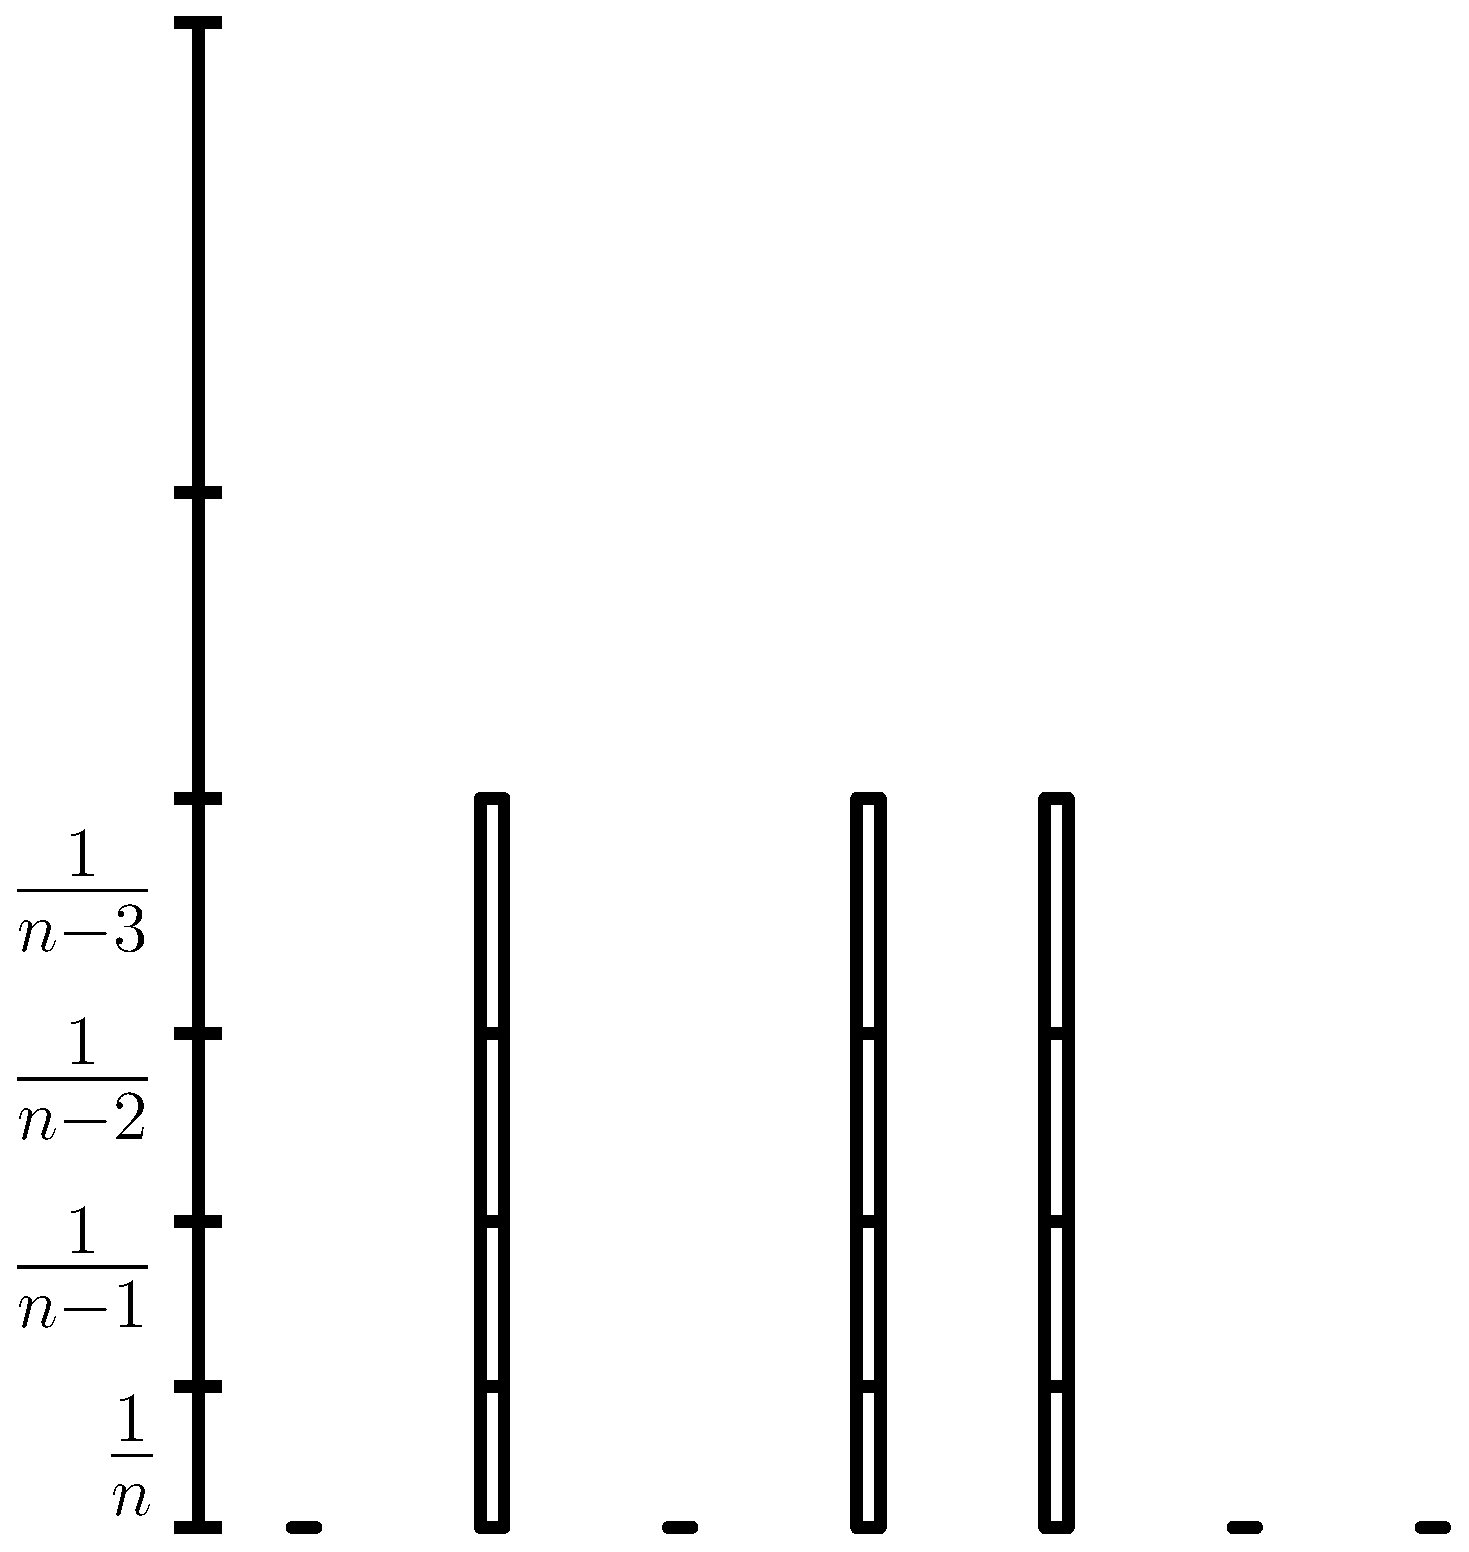
\includegraphics[width=0.5\linewidth]{singleProcessorLowerBound/round_4_1.eps}
    \onslide<10>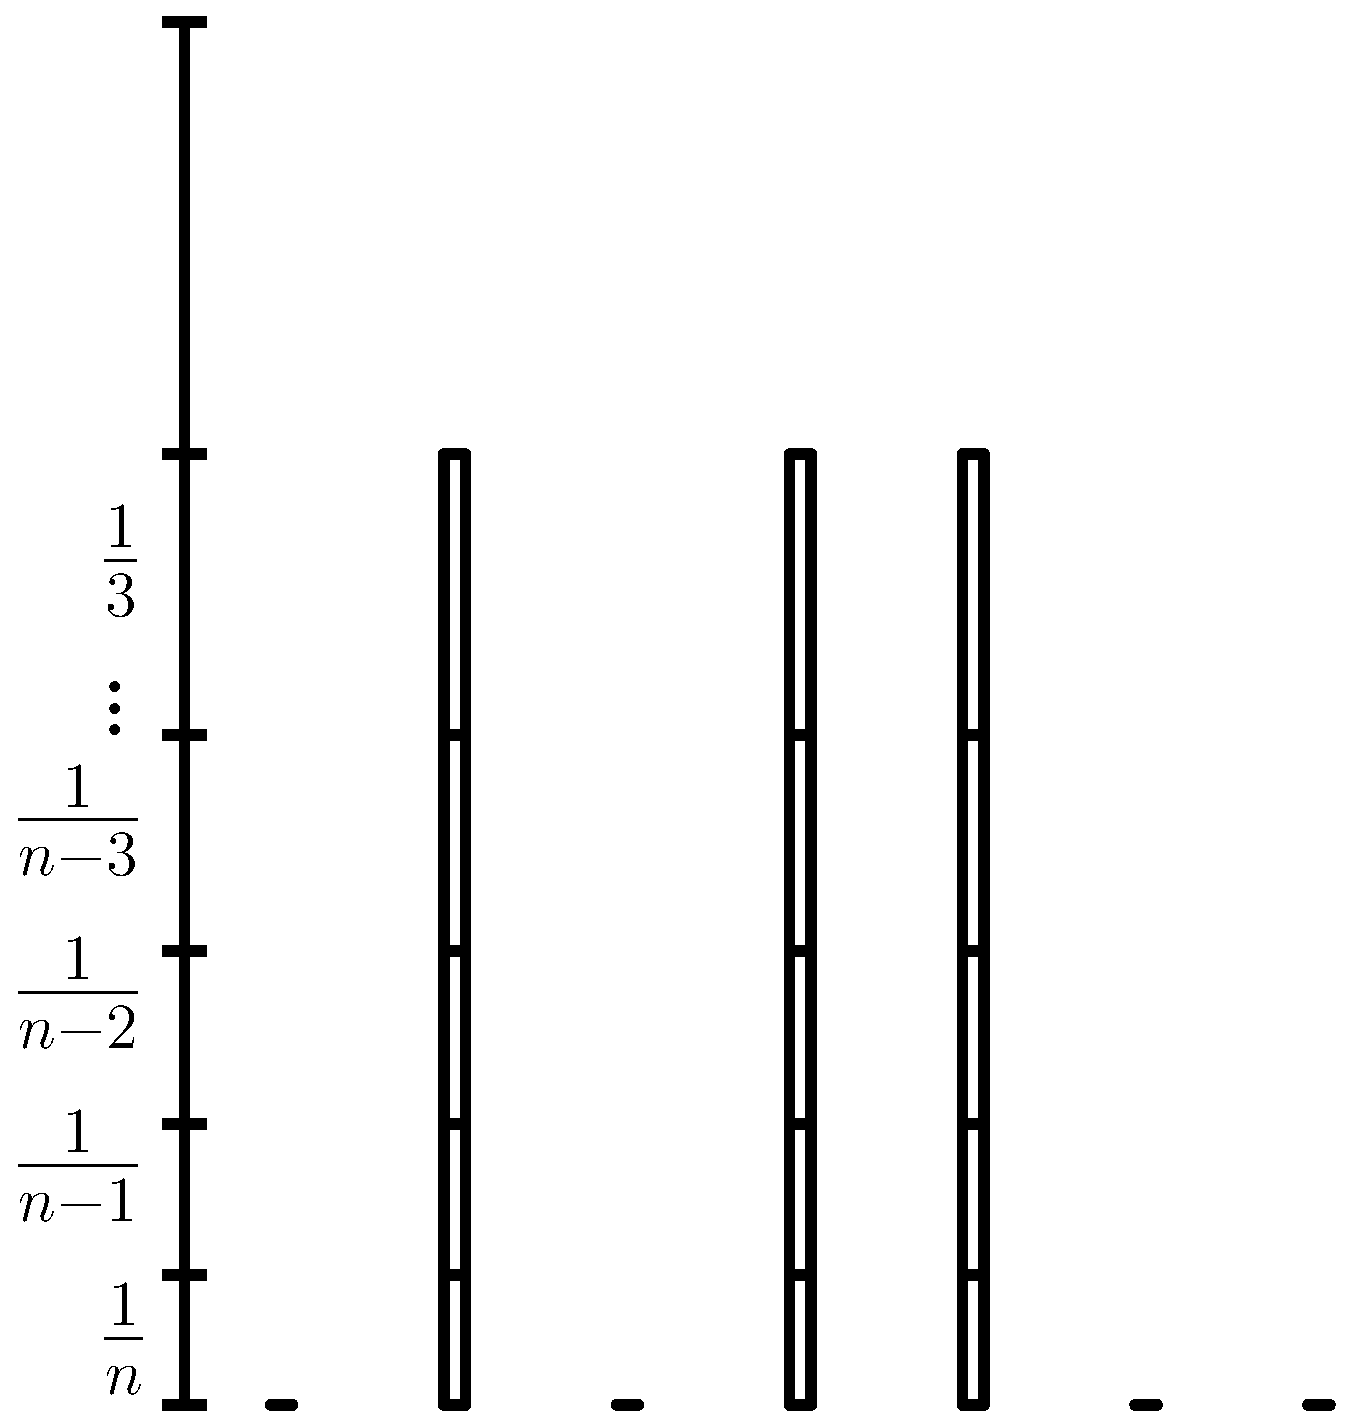
\includegraphics[width=0.5\linewidth]{singleProcessorLowerBound/round_5_0.eps}
    \onslide<11>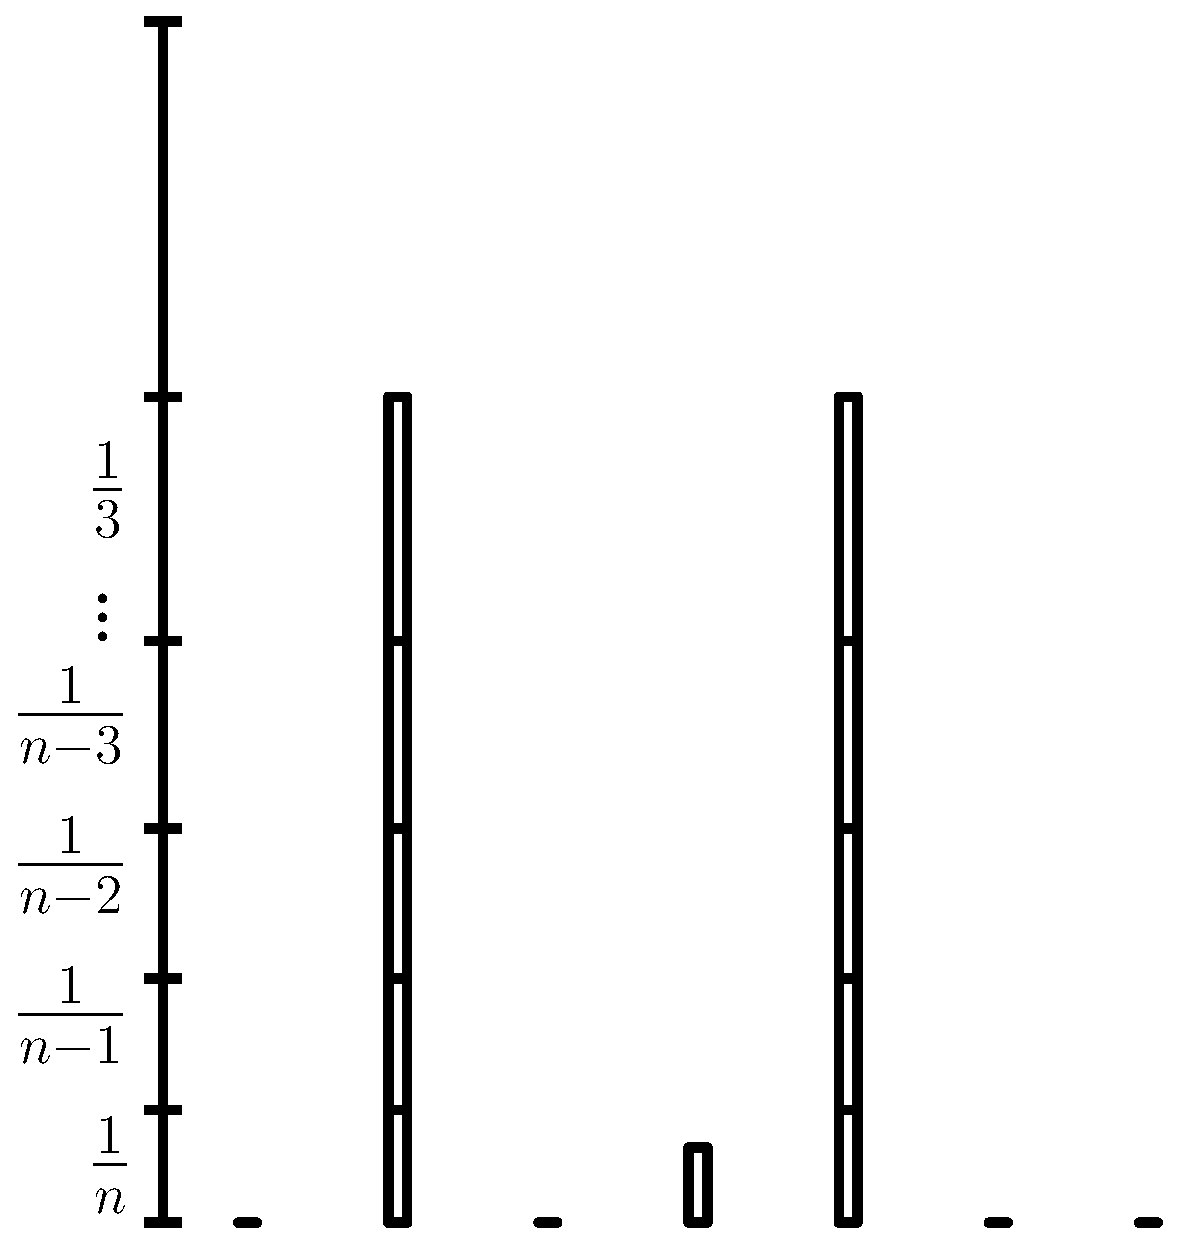
\includegraphics[width=0.5\linewidth]{singleProcessorLowerBound/round_5_1.eps}
    \onslide<12>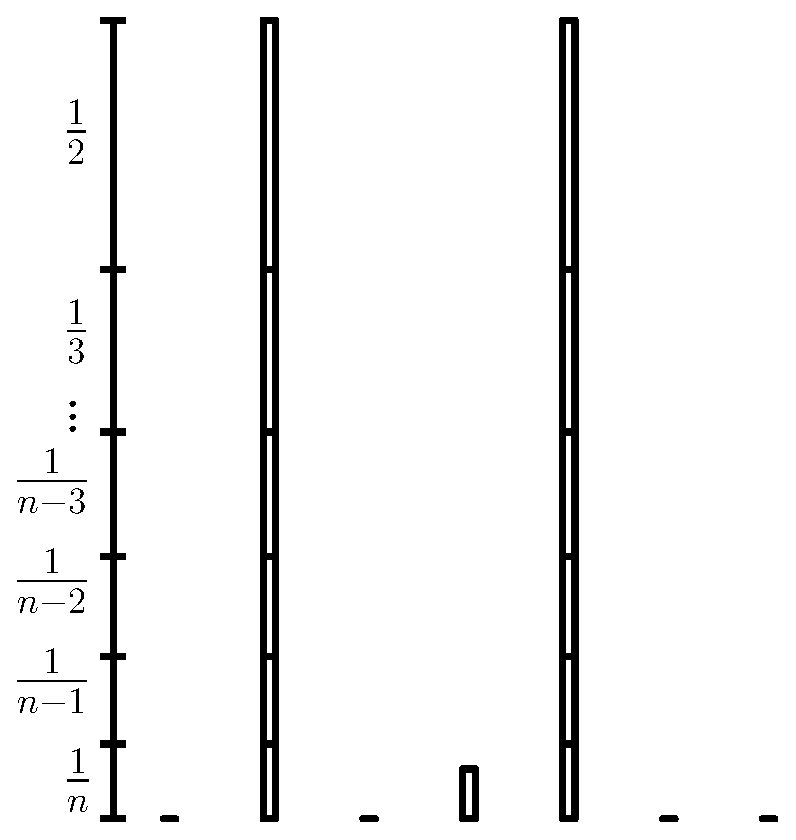
\includegraphics[width=0.5\linewidth]{singleProcessorLowerBound/round_6_0.eps}
    \onslide<13>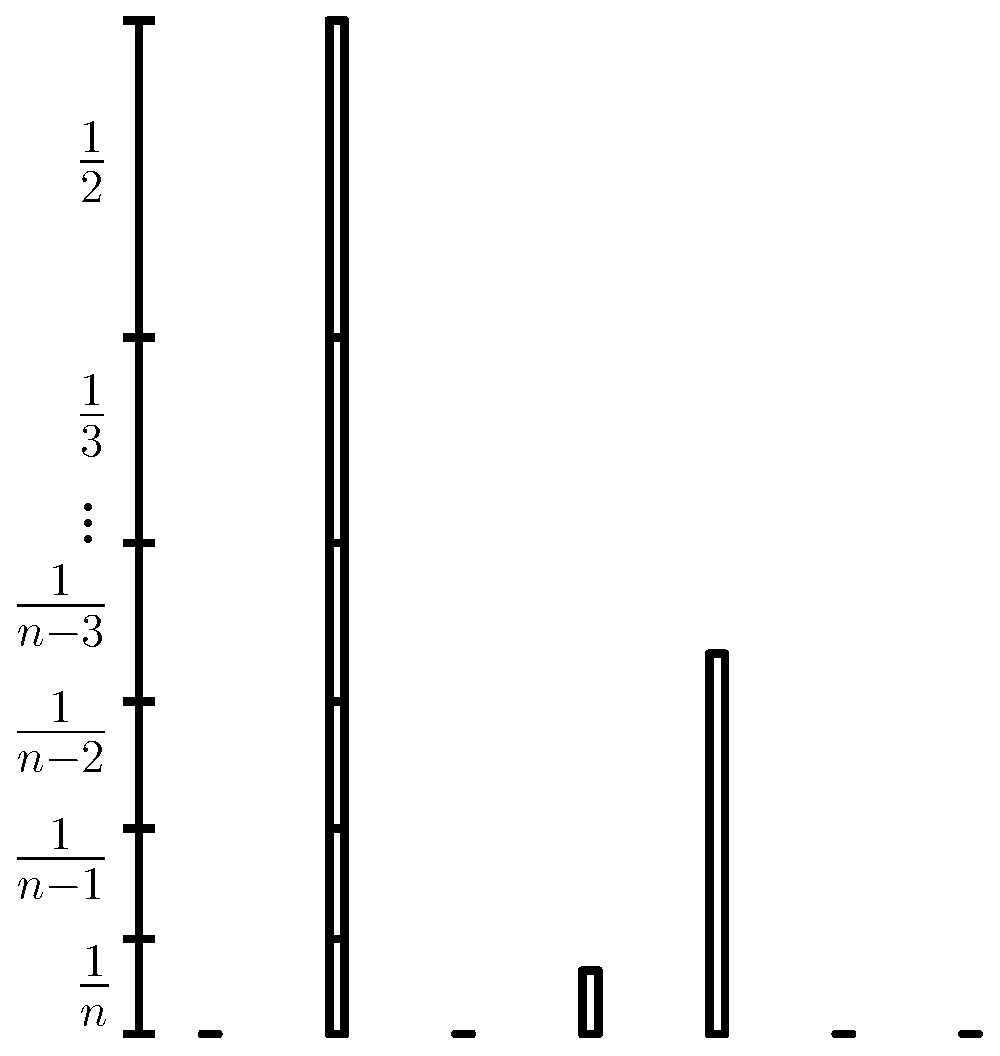
\includegraphics[width=0.5\linewidth]{singleProcessorLowerBound/round_6_1.eps}
    \onslide<14>\vspace{1.5cm}Achieves backlog: $$\frac{1}{n} + \frac{1}{n-1} + \cdots + \frac{1}{2} = \Omega(\log n).$$ 
  \end{overprint}
\end{frame}

\begin{frame}[t]{Single-Processor Upper Bound}
  A \defn{greedy emptier} -- an emptier that always empties from the
    fullest cup -- never lets backlog exceed $O(\log n)$.

  \vspace{0.75cm}
  \begin{definitions}
  \begin{itemize}
    \item Let $S_t$ denote the cup state at the start of round $t$
    \item Let $I_t$ denote the state after the filler has added water on round $t$ but before the emptier has emptied from cups
    \item Let $\mu_k(S_t)$ denote the average fill of the $k$ fullest cups in $S_t$.
  \end{itemize}
  \end{definitions}
\end{frame}

\begin{frame}[t]{Single-Processor Upper Bound Proof}
  \textbf{Proof:}
  Inductively prove a set of invariants: 
    $$\mu_k(S_t) \le \frac{1}{k+1} + \ldots \frac{1}{n}.$$

  \vspace{0.25cm}
  Let $a$ be the cup that the emptier empties from in state $S_{t}$.

  \vspace{0.25cm}
  \textbf{Case 1: $a$ is the fullest cup in $S_{t+1}$}\\
  $$\mu_k(S_{t+1}) \le \mu_k(S_t).$$

  \vspace{0.25cm}
  \textbf{Case 2: $a$ is not the fullest cup in $S_{t+1}$}
  $$\mu_k(S_{t+1}) \le \mu_{k+1}(I_t) \le \mu_{k+1}(S_{t+1}) + \frac{1}{k+1}.$$
\end{frame}

\begin{frame}[t]{Previous work on Cup Games}
  \begin{itemize}
    \item The Single-Processor cup game ($p=1$) has been tightly analyed with
      \defn{oblivious} and \defn{adaptive} fillers (i.e. fillers that can't and
      can observe the emtpier's actions).
    \item The Multi-Processor cup game ($p>1$) is substantially more difficult. With an adaptive filler:
      \begin{itemize}
        \item Kuszmaul established upper bound of $O(\log n)$.\footnote{\tiny\color{blue}William Kuszmaul. Achieving optimal backlog in the vanilla multi-processor cup game. SIAM, 2020.}
        \item We established a matching lower bound of $\Omega(\log n)$.
      \end{itemize}
    \item The multi-processor cup game with an oblivious filler has not yet
      been tightly analyzed.
    \item Variants where valid moves depend on a graph have been studied.
    \item Variants with resource augmentation have been studied.
    \item Variants with clairvoyance have been studied.
  \end{itemize}
\end{frame}

\begin{frame}[t]{Our Variant of the Cup Game}
We investigate a variant of the classic multi-processor cup game,
the \defn{variable-processor cup game}, in which \emph{the resources are variable}:
the filler is allowed to change $p$.

\vspace{1cm}
Although the modification to allow variable resources seems small, we will
show that it drastically alters the outcome of the game.
\end{frame}

\begin{frame}[t]{Amplification Lemma}
  \begin{lemma}
    Given a filling strategy for achieving backlog $f(n)$ on $n$ cups, we can construct a new filling strategy that achieves backlog 
    $$f'(n) \ge (1-\delta)\sum_{\ell=0}^L f((1-\delta)\delta^\ell n)$$
    for any parameter $\delta$ with $0 < \delta \ll 1/2$ of our choice, where $L$
    is the largest integer such that we can achieve backlog $1$ on
    $(1-\delta)\delta^Ln$ cups.%, i.e. $L = \frac{\log n + O(1)}{\log 1/\delta}$.
  \end{lemma}
  Remark: WLOG the number of cups in the recursive calls is an integer.
  
\end{frame}

\begin{frame}[t]{Proof Sketch of Amplification Lemma}
  \begin{itemize}
    \item Let $A$ be the $\delta n$ fullest cups and $B$ be the $(1-\delta)n$ other cups.
    \item By repeatedly applying $f$ to each cup in $B$, and transfering over
      the cup generated in $B$ with backlog $f((1-\delta)n)$ to $A$, while maintaining the fill of cups in $A$, we make
      $\mu (A) - \mu (B) \ge f((1-\delta)n)$. This is accomplished while
      maintaining $\mu(A\cup B)$. The mass of $A$ is guaranteed to be obve
      $a\mu(A\cup B)$ by the same amount that the mass of $B$ is guaranteed to
      be depressed from $b\mu(A\cup B)$, thus fraction of the difference that
      $\mu(A)$ gets is $|B|/|A\cup B| = (1-\delta)$. So $\mu(A)$ is at least
      $(1-\delta)f((1-\delta)n)$ above $\mu(A\cup B)$.
    \item We then recursively apply this procedure to $A$. Summing over $\ell = 0,1, \ldots, L$ we have the desired result.
  \end{itemize} 

  Note: we are ignoring a lot of details here, e.g. ensuring that we actually are playing a cup game on $B$ when applying $f$ to it.
\end{frame}

\begin{frame}[t]{Lower Bound against Adaptive Filler}
  Setting $\delta = O(1/n)$ and analyzing a filling strategy that  recursively
  applies the Amplification Lemma we proved
  \begin{corollary}
    The filler can achieve backlog 
    $$\Omega(n)$$
  \end{corollary}
\end{frame}

\begin{frame}[t]{Upper Bound against Adaptive Filler}
  We prove a novel set of invariants:

  \begin{theorem}
    A greedy emptier maintains the invariant:
    $$\mu_k(S_t) \le n-k.$$
  \end{theorem}

  \vspace{0.3cm}
  In particular this implies that backlog is $$O(n).$$

  \vspace{0.3cm}
  Note: this matches our lowerbound!
  
\end{frame}

\begin{frame}[t]{Strategy Even Works with Oblivious filler!}
  Using Hoeffding's Concentration Inequality\footnote{\tiny\color{blue} Wassily
  Hoeffding. Probability inequalities for sums of bounded random variables.
Journal of the American Statistical Association, page 28, 1962.}, we can
surprisingly prove the same lower-bound for an Oblivious filler as for an
Adaptive filler, although only against \defn{greedy-like} emptiers.
\end{frame}

\begin{frame}[t]{Open Questions}
  \begin{itemize}
    \item Can we extend the Oblivious lower-bound construction to work against a broader class of emptiers?
    \item Can we extend the Oblivious lower-bound construction to work against arbitrary emptiers?
  \end{itemize}
\end{frame}

\begin{frame}[t]{Acknowledgements}
  \begin{itemize}
    \item My mentor, William Kuszmaul!
    \item MIT PRIMES
    \item My Parents
 \end{itemize} 
\end{frame}

\end{document}
